\documentclass{beamer}
\usetheme{Antibes}
\usecolortheme{orchid}
\usepackage{amsmath}
\usepackage[utf8]{inputenc}
\usepackage{tikz}
\usepackage{graphicx}
\usetikzlibrary{matrix}
\graphicspath{ {./} }

\def\insertauthorindicator{Who?}% Default is "Who?"
\def\insertinstituteindicator{From?}% Default is "From?"
\def\insertdateindicator{When?}% Default is "When?"

\title{Neural networks}
\subtitle{Architectures and training tips}

\author{Sebastian Bj{\"o}rkqvist}
\institute{IPRally Technologies}

\date[09.01.2019]{09.01.2019}

\newcommand{\kur}{\protect\textit}
\newcommand{\bol}{\protect\textbf}
\newcommand\pro{\item[$+$]}
\newcommand\con{\item[$-$]}

\def\layersep{2.2cm}
\begin{document}
\setbeamertemplate{caption}{\raggedright\insertcaption\par}

\frame{\titlepage}
  \begin{frame}
    \frametitle{What is a neural network?}  
    
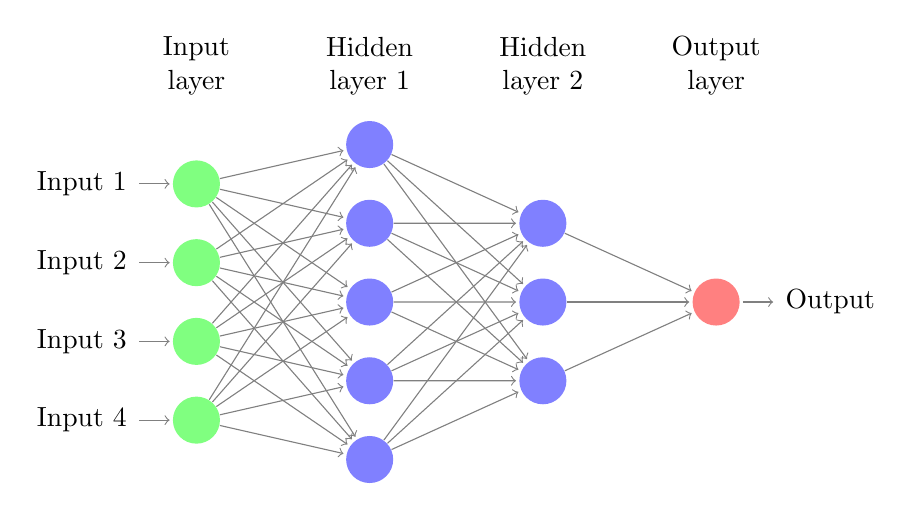
\begin{tikzpicture}[shorten >=1pt,->,draw=black!50, node distance=\layersep]
    \tikzstyle{every pin edge}=[<-,shorten <=1pt]
    \tikzstyle{neuron}=[circle,fill=black!25,minimum size=17pt,inner sep=0pt]
    \tikzstyle{input neuron}=[neuron, fill=green!50];
    \tikzstyle{output neuron}=[neuron, fill=red!50];
    \tikzstyle{hidden neuron}=[neuron, fill=blue!50];    
    \tikzstyle{hidden neuron 2}=[neuron, fill=blue!50];
    \tikzstyle{annot} = [text width=4em, text centered]

    % Draw the input layer nodes
    \foreach \name / \y in {1,...,4}
    % This is the same as writing \foreach \name / \y in {1/1,2/2,3/3,4/4}
        \node[input neuron, pin=left:Input \y] (I-\name) at (0,-\y) {};

    % Draw the hidden layer nodes
    \foreach \name / \y in {1,...,5}
        \path[yshift=0.5cm]
            node[hidden neuron] (H-\name) at (\layersep,-\y cm) {};

    % Draw the hidden layer nodes
    \foreach \name / \y in {1,...,3}
        \path[yshift=-0.5cm]
            node[hidden neuron 2] (F-\name) at (2*\layersep,-\y cm) {};

    % Draw the output layer node
    \node[output neuron,pin={[pin edge={->}]right:Output}, right of=F-2] (O) {};

    % Connect every node in the input layer with every node in the
    % hidden layer.
    \foreach \source in {1,...,4}
        \foreach \dest in {1,...,5}
            \path (I-\source) edge (H-\dest);
    \foreach \source in {1,...,5}
        \foreach \dest in {1,...,3}
            \path (H-\source) edge (F-\dest);

    % Connect every node in the hidden layer with the output layer
    \foreach \source in {1,...,3}
        \path (F-\source) edge (O);

    % Annotate the layers
    \node[annot,above of=H-1, node distance=1cm] (hl) {Hidden layer 1};
    \node[annot,right of=hl, node distance=\layersep] (fl) {Hidden layer 2};
    \node[annot,left of=hl] {Input layer};
    \node[annot,right of=fl] {Output layer};
\end{tikzpicture}

  \tiny Modified from \url{http://www.texample.net/tikz/examples/neural-network/}
  \end{frame}

  \begin{frame}
    \frametitle{What is a neural network?}  
    At each hidden layer node $i$ the output value is calculated by 
	\begin{align*}
    o_{i} = f(\sum{w_{ki}o_{ki-1}} + b_{i}). 
    \end{align*}
    \onslide<2->{The function $f$ is called the activation function. It must be non-linear to allow the network to learn non-linear dependencies.}
  \end{frame} 
  \begin{frame}
    \frametitle{Training neural networks using SGD}  
  
  \begin{figure}[sgd]
    \vspace*{-0.4cm}
  	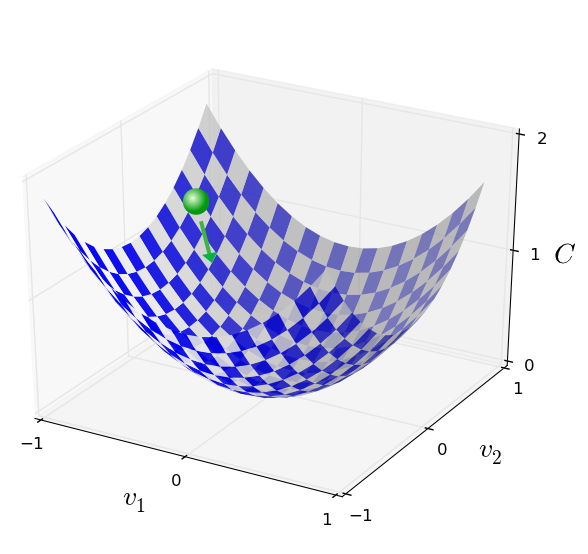
\includegraphics[scale=0.22]{sgd_visualization} 
  	\centering
	\caption{\tiny \cite{nielsen}, Chapter 1.}  	
  \end{figure}

	
	The training data is processed in small batches, and the weights of the model are iteratively updated by going in the direction of the negative gradient of the loss function.
  \end{frame}  
  \begin{frame}
    \frametitle{Why neural networks?}  
    
   	\begin{itemize}
		\item Can approximate any function \cite{hornik}
		\onslide<2->{\item May learn to respond to unexpected patterns}
		\onslide<3->{\item Useful especially when the amount of data is large compared to input dimensionality}
		\onslide<4->{\item Less need for feature engineering compared to traditional ML methods}
	\end{itemize}
  \end{frame}
  
  \begin{frame}
    \frametitle{Recurrent neural network (RNN)}  
    
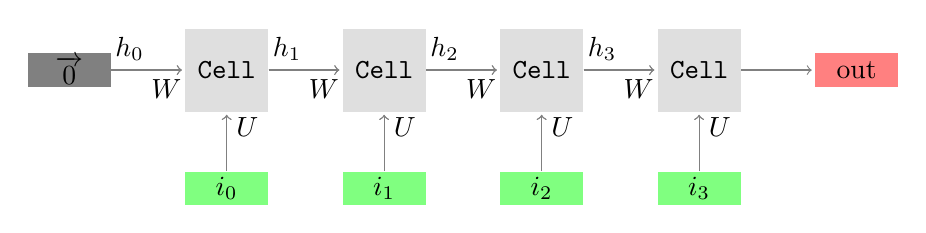
\begin{tikzpicture}[shorten >=1pt,->,draw=black!50, node distance=\layersep]
    \tikzstyle{every pin edge}=[<-,shorten <=1pt]
    \tikzstyle{vector}=[rectangle,fill=black!25,minimum width =30pt, minimum height=12pt,inner sep=0pt]    
    \tikzstyle{cell}=[rectangle,fill=gray!25,minimum width =30pt, minimum height=30pt,inner sep=0pt, font=\ttfamily]
    \tikzstyle{input vector}=[vector, fill=green!50];
    \tikzstyle{hidden vector}=[vector, fill=blue!50];
    \tikzstyle{output vector}=[vector, fill=red!50];
    \tikzstyle{zero vector}=[vector, fill=black!50];        
    \tikzstyle{annot} = [text width=4em, text centered]

        \node[zero vector] (H-0) at (0,-1) {$\overrightarrow{0}$};
        \foreach \name / \y in {1,...,4}
        	\node[cell] (C-\y) at (2*\y,-1) {Cell};
        \foreach \name / \y in {0,...,3}
        	\node[input vector] (I-\y) at (2*\y + 2,-2.5) {$i_{\y}$};
        \node[output vector] (O) at (10,-1) {out};

	\path (H-0) edge node[near start, above] {$h_{0}$} (C-1);
	\path (H-0) edge node[near end, below] {$\bold{W}$} (C-1);
	
    \foreach \y [count=\i] in {2,...,4}
    	\path (C-\i) edge node[near start, above] {$h_{\i}$}(C-\y);
    \foreach \y [count=\i] in {2,...,4}
    	\path (C-\i) edge node[near end, below] {$\bold{W}$}(C-\y);

	\path (C-4) edge (O);
	
	\foreach \y [count=\i] in {0,...,3}
		\path (I-\y) edge (C-\i); 
	\foreach \y [count=\i] in {0,...,3}
		\path (I-\y) edge node[near end, right]{$\bold{U}$}(C-\i);   	


\end{tikzpicture}  
	
	Processes each element of the input sequence in order, and keeps information about the past elements in a hidden state vector.

  \end{frame}  
  
  \begin{frame}
    \frametitle{Recurrent neural network (RNN)}  
    
	At each timestep $t$ the new hidden state is calculated using the new input at this timestep and the existing hidden state. The most basic version is the following:
	
	\begin{align*}
    h_{t} = \sigma(Wh_{t-1} + Ui_{t} + b). 
    \end{align*}	
	
  \onslide<2->{Other RNN architectures (for instance LSTM or GRU) use more complicated ways of updating the hidden state to control the flow of information to and from the hidden state.}
  \end{frame}      
  
  \begin{frame}
    \frametitle{RNN pros and cons}  
    
   	\begin{itemize}
		\onslide<2->{\pro Accepts input of variable size, i.e. sequences (time series, sentences etc)}
		\onslide<3->{
		\begin{itemize}
				\item{Can even be used to process tree-structured inputs by using Tree-LSTMs \cite{tai}}
		\end{itemize}}			
		\onslide<4->{\pro May learn long-term dependencies, especially when using LSTM architecture}
		\onslide<5->{\con Training may be slow when sequence length is large}		
		\onslide<6->{
		\begin{itemize}
				\item{This is because each time step depends on the earlier ones and they must thus be processed sequentially}
		\end{itemize}}
		\onslide<7->{\con Prediction accuracy may also suffer if the sequence is long}						\onslide<8->{
		\begin{itemize}
				\item{The model may not remember early inputs and can be biased toward the end of the sequence}
		\end{itemize}}
		
	\end{itemize}
  \end{frame}    

  \begin{frame}
    \frametitle{RNN real life use case: Patent search}  
    
	At IPRally we work on automated patent searches. The basic idea is the following:
	
	\begin{enumerate}
		\onslide<2->{\item Patents are transformed to graphs by extracting the relevant information from the patent claims and specifications}
		\onslide<3->{\item The graphs are then embedded to vectors by using a Tree-LSTM model}
		\begin{itemize}
			\onslide<4->{\item {The model is trained by using millions of real-life positive and negative novelty citations from previous patent applications}}
			\onslide<5->{\item {Patents with a positive citation get vectors that are close to each other}}
		\end{itemize}
		\onslide<6->{\item A prior art search for a new patent can then be done by searching for the nearest neighbors of the vector created from the new invention}
	\end{enumerate}

  \end{frame}    

  \begin{frame}
    \frametitle{RNN real life use case: Patent search}  
  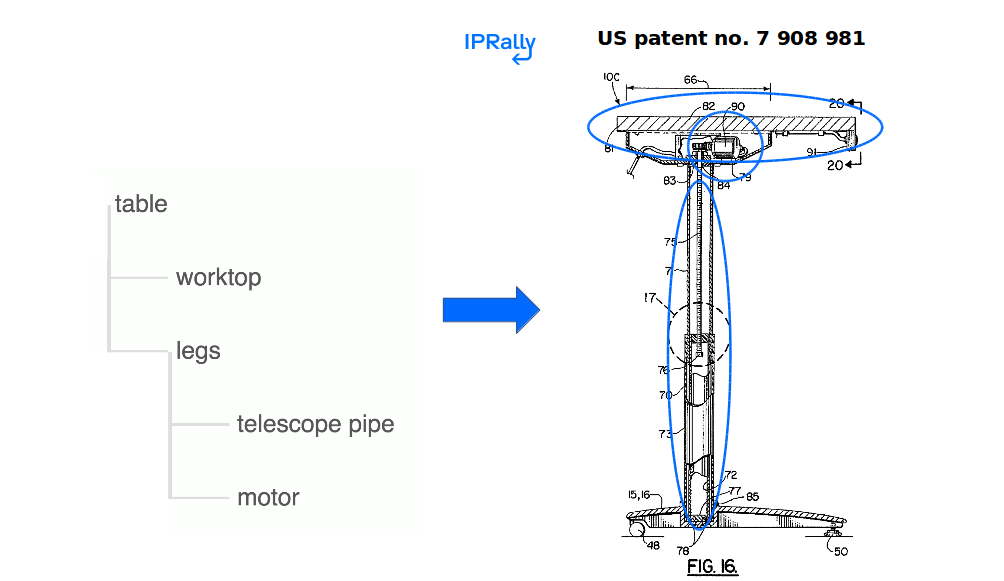
\includegraphics[scale=0.32]{patent_search_iprally_slide_20190106} 
  \end{frame}

  \begin{frame}
    \frametitle{Convolutional neural network (CNN)}  
    
  Feed-forward networks do not scale well to images due to the large input size. Convolutional neural networks are constrained to looking only at a small part of the image at a time, and thus the number of weights stays manageable.
   \vspace{8mm}
  
  A CNN uses three types of layers: convolutional, pooling and fully connected. 
  

  \end{frame}  
  
  \begin{frame}
    \frametitle{CNN - Convolutional layer}  
	   	\begin{itemize}
		\onslide<2->{\item Consists of a set of learnable filters}
		\onslide<3->{\item Each individual filter is small (i.e. small height and width)}
		\onslide<4->{\item During the forward pass we slide each filter across the entire input and compute dot products between input entries and filter weights}
		\onslide<5->{\item The idea is that each filter learns to identify some kind of feature (for instance part of a shape)}
	\end{itemize}
  \end{frame}   
  
  \begin{frame}
    \frametitle{CNN - Convolutional layer}  
    
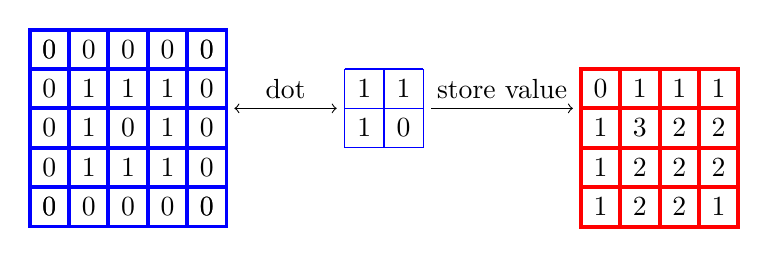
\begin{tikzpicture}
\draw[step=0.5cm,color=gray] (-1,-1) grid (1.5,1.5);

\foreach \y in {+1.25,+0.75,+0.25,-0.25,-0.75}
{
	\node at (-0.75,\y) {0};
    \node at (1.25,\y) {0};
}
\foreach \x in {+1.25,+0.75,+0.25,-0.25,-0.75}
{
	\node at (\x,-0.75) {0};
    \node at (\x, 1.25) {0};
}
\foreach \x in {+0.75,+0.25,-0.25}
{
	\node at (\x,-0.25) {1};
    \node at (\x, 0.75) {1};
}
	\node at (-0.25,0.25) {1};
    \node at (0.75, 0.25) {1};
	\node at (0.25,0.25) {0};    

\onslide<2->{
\draw[step=0.5cm,color=blue] (3-0.001,-0.001) grid (4,1);
	\node at (3.75,0.25) {0};	
	\node at (3.75,0.75) {1};	
	\node at (3.25,0.25) {1};	
	\node at (3.25,0.75) {1};
\draw[step=0.5cm,color=red] (6-0.001,-1-0.001) grid (8,1);	
}
\onslide<3->{   \path[<->] (1.6,0.5) edge node[above] {dot} (2.9,0.5);
}
\onslide<3-4>{
\draw[step=0.5cm,color=blue, line width=0.5mm] (-1,0.5) rectangle (0,1.5);


}
\onslide<4->{
	\path[->] (4.1,0.5) edge node[above] {store value}(5.9,0.5);
\node at (6.25,0.75) {0};
}
\onslide<4-4>{
\draw[step=0.5cm,color=red, line width=0.5mm] (6-0.001,0.5-0.001) rectangle (6.5,1);	
}
\onslide<5-5>{
\draw[step=0.5cm,color=blue, line width=0.5mm] (-0.5,0.5) rectangle (0.5,1.5);
\draw[step=0.5cm,color=red, line width=0.5mm] (6.5-0.001,0.5-0.001) rectangle (7,1);
}
\onslide<5->{
\node at (6.75,0.75) {1};
}
\onslide<6-6>{
\draw[step=0.5cm,color=blue, line width=0.5mm] (0,0.5) rectangle (1,1.5);
\draw[step=0.5cm,color=red, line width=0.5mm] (7-0.001,0.5-0.001) rectangle (7.5,1);
}
\onslide<6->{
\node at (7.25,0.75) {1};
}
\onslide<7-7>{
\draw[step=0.5cm,color=blue, line width=0.5mm] (0.5,0.5) rectangle (1.5,1.5);
\draw[step=0.5cm,color=red, line width=0.5mm] (7.5-0.001,0.5-0.001) rectangle (8,1);
}
\onslide<7->{
\node at (7.75,0.75) {1};
}
\onslide<8-8>{
\draw[step=0.5cm,color=blue, line width=0.5mm] (-1,0) rectangle (0,1);
\draw[step=0.5cm,color=red, line width=0.5mm] (6-0.001,0-0.001) rectangle (6.5,0.5);
}
\onslide<8->{
\node at (6.25,0.25) {1};
}
\onslide<9-9>{
\draw[step=0.5cm,color=blue, line width=0.5mm] (-0.5,0) rectangle (0.5,1);
\draw[step=0.5cm,color=red, line width=0.5mm] (6.5-0.001,0-0.001) rectangle (7,0.5);
}
\onslide<9->{
\node at (6.75,0.25) {3};
}
\onslide<10-10>{
\draw[step=0.5cm,color=blue, line width=0.5mm] (0,0) rectangle (1,1);
\draw[step=0.5cm,color=red, line width=0.5mm] (7-0.001,0-0.001) rectangle (7.5,0.5);
}
\onslide<10->{
\node at (7.25,0.25) {2};
}
\onslide<11-11>{
\draw[step=0.5cm,color=blue, line width=0.5mm] (0.5,0) rectangle (1.5,1);
\draw[step=0.5cm,color=red, line width=0.5mm] (7.5-0.001,0-0.001) rectangle (8,0.5);
}
\onslide<11->{
\node at (7.75,0.25) {2};
}
\onslide<12-12>{
\draw[step=0.5cm,color=blue, line width=0.5mm] (-1,-0.5) rectangle (0,0.5);
\draw[step=0.5cm,color=red, line width=0.5mm] (6-0.001,-0.5-0.001) rectangle (6.5,0);
}
\onslide<12->{
\node at (6.25,-0.25) {1};
}
\onslide<13-13>{
\draw[step=0.5cm,color=blue, line width=0.5mm] (-0.5,-0.5) rectangle (0.5,0.5);
\draw[step=0.5cm,color=red, line width=0.5mm] (6.5-0.001,-0.5-0.001) rectangle (7,0);
}
\onslide<13->{
\node at (6.75,-0.25) {2};
}
\onslide<14-14>{
\draw[step=0.5cm,color=blue, line width=0.5mm] (0,-0.5) rectangle (1,0.5);
\draw[step=0.5cm,color=red, line width=0.5mm] (7-0.001,-0.5-0.001) rectangle (7.5,0);
}
\onslide<14->{
\node at (7.25,-0.25) {2};
}
\onslide<15-15>{
\draw[step=0.5cm,color=blue, line width=0.5mm] (0.5,-0.5) rectangle (1.5,0.5);
\draw[step=0.5cm,color=red, line width=0.5mm] (7.5-0.001,-0.5-0.001) rectangle (8,0);
}
\onslide<15->{
\node at (7.75,-0.25) {2};
}
\onslide<16-16>{
\draw[step=0.5cm,color=blue, line width=0.5mm] (-1,-1) rectangle (0,0);
\draw[step=0.5cm,color=red, line width=0.5mm] (6-0.001,-1-0.001) rectangle (6.5,-0.5);
}
\onslide<16->{
\node at (6.25,-0.75) {1};
}
\onslide<17-17>{
\draw[step=0.5cm,color=blue, line width=0.5mm] (-0.5,-1) rectangle (0.5,0);
\draw[step=0.5cm,color=red, line width=0.5mm] (6.5-0.001,-1-0.001) rectangle (7,-0.5);
}
\onslide<17->{
\node at (6.75,-0.75) {2};
}
\onslide<18-18>{
\draw[step=0.5cm,color=blue, line width=0.5mm] (0,-1) rectangle (1,0);
\draw[step=0.5cm,color=red, line width=0.5mm] (7-0.001,-1-0.001) rectangle (7.5,-0.5);
}
\onslide<18->{
\node at (7.25,-0.75) {2};
}
\onslide<19-19>{
\draw[step=0.5cm,color=blue, line width=0.5mm] (0.5,-1) rectangle (1.5,0);
\draw[step=0.5cm,color=red, line width=0.5mm] (7.5-0.001,-1-0.001) rectangle (8,-0.5);
}
\onslide<19->{
\node at (7.75,-0.75) {1};
}
\end{tikzpicture}

  \end{frame}     
  \begin{frame}
    \frametitle{CNN - Pooling layer}  
	   	\begin{itemize}
		\onslide<2->{\item Reduces the size of the representation by summarizing parts of the input}		\begin{itemize}
			\onslide<3->{\item {This is done to decrease the amount of computation in the network}}\end{itemize}
		\onslide<4->{\item A common way is to take the maximum value of a small grid (max pooling)}
		\begin{itemize}
			\onslide<5->{\item {For instance if we use max pooling with a filter of size 2x2 we discard 75 percent of the values}}
			\end{itemize}
	\end{itemize}
  \end{frame}     
  
   
  \begin{frame}
    \frametitle{CNN - Pooling layer}  
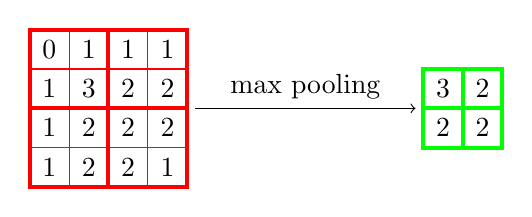
\begin{tikzpicture}
\draw[step=0.5cm,color=red] (-0.001,-1-0.001) grid (2,1);	
\node at (0.25,0.75) {0};
\node at (0.75,0.75) {1};
\node at (1.25,0.75) {1};
\node at (1.75,0.75) {1};
\node at (0.25,0.25) {1};
\node at (0.75,0.25) {3};
\node at (1.25,0.25) {2};
\node at (1.75,0.25) {2};
\node at (0.25,-0.25) {1};
\node at (0.75,-0.25) {2};
\node at (1.25,-0.25) {2};
\node at (1.75,-0.25) {2};
\node at (0.25,-0.75) {1};
\node at (0.75,-0.75) {2};
\node at (1.25,-0.75) {2};
\node at (1.75,-0.75) {1};

\onslide<2-3>{
\draw[step=0.5cm,color=red, line width=0.5mm] (0-0.001,0-0.001) rectangle (1,1);
}
\onslide<2->{
\draw[step=0.5cm,color=green] (5-0.001,-0.5-0.001) grid (6,0.5);
}
\onslide<3->{
\path[->] (2.1,0) edge node[above] {max pooling}(4.9,0);
\node at (5.25,0.25) {3};
}
\onslide<3-3>{
\draw[step=0.5cm,color=green, line width=0.5mm] (5-0.001,0.001) rectangle (5.5,0.5);
}
\onslide<4->{
\node at (5.75,0.25) {2};
}
\onslide<4-4>{
\draw[step=0.5cm,color=red, line width=0.5mm] (1-0.001,0-0.001) rectangle (2,1);

\draw[step=0.5cm,color=green, line width=0.5mm] (5.5-0.001,0.001) rectangle (6,0.5);
}
\onslide<5->{
\node at (5.25,-0.25) {2};
}
\onslide<5-5>{
\draw[step=0.5cm,color=red, line width=0.5mm] (0-0.001,-1-0.001) rectangle (1,0);

\draw[step=0.5cm,color=green, line width=0.5mm] (5-0.001,-0.5-0.001) rectangle (5.5,0);
}
\onslide<6->{
\node at (5.75,-0.25) {2};
}
\onslide<6-6>{
\draw[step=0.5cm,color=red, line width=0.5mm] (1-0.001,-1-0.001) rectangle (2,0);

\draw[step=0.5cm,color=green, line width=0.5mm] (5.5-0.001,-0.5-0.001) rectangle (6,0);
}
\end{tikzpicture}
  \end{frame}    
    
  \begin{frame}
    \frametitle{CNN - Example architecture}  
  \begin{figure}[convnet]
  	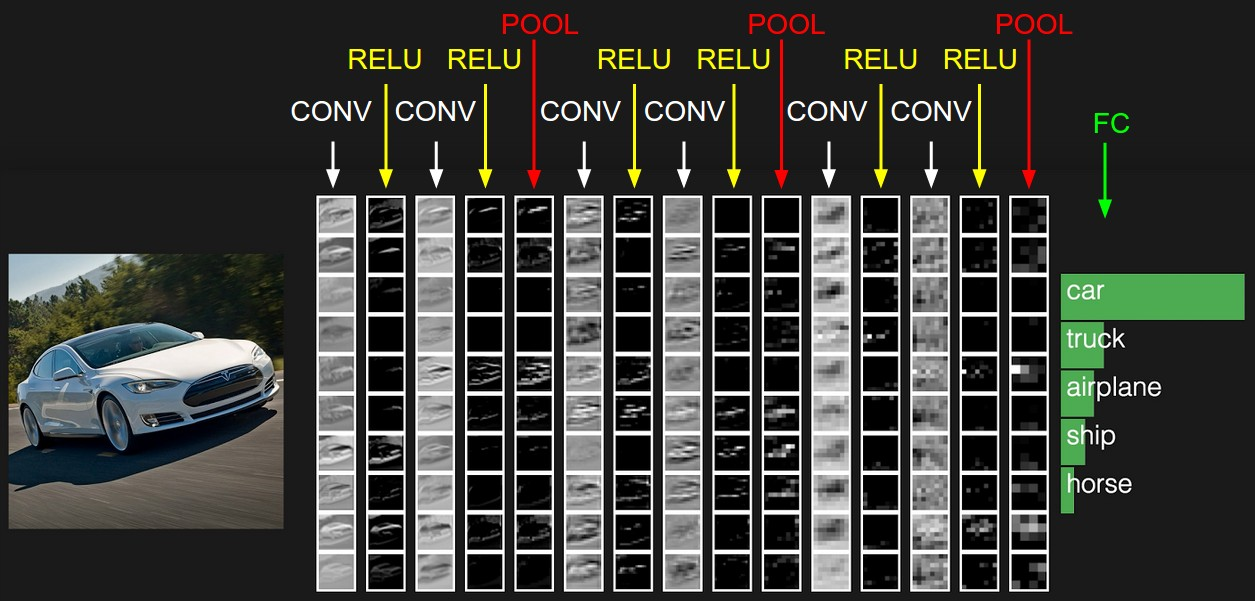
\includegraphics[scale=0.25]{convnet} 
  	\centering
	\caption{\tiny Taken from \url{http://cs231n.github.io/convolutional-networks/}}  	
  \end{figure}
  \end{frame}      
  
  \begin{frame}
    \frametitle{CNN pros and cons}  
    
   	\begin{itemize}
		\onslide<2->{\pro Works well with image data and text data}
		\onslide<3->{\pro Training can be effectively parallelized}
		\onslide<4->{\pro Pre-existing models can be fine-tuned for specific tasks}
		\onslide<5->{\con Does not take into account orientation of the object}
	\end{itemize}
  \end{frame}    

  \begin{frame}
    \frametitle{Challenges when training neural networks}  
    
   	\begin{itemize}
		\onslide<2->{\item Finding the optimal neural network layout is often time-consuming}
		\onslide<3->{\item The model may be sensitive to changes in hyperparameters, especially learning rate and activation function}
		\onslide<4->{\item A model may take several hours or even days to train}
		\onslide<4->{
		\begin{itemize}
				\item{This makes hyperparameter searches very expensive}
		\end{itemize}}			
		\onslide<5->{\item It's often hard to know why the model predicts as it does because of the complexity of the model}	
		

	\end{itemize}
  \end{frame}  

  \begin{frame}
    \frametitle{Tips and tricks}  
    
   	\begin{itemize}
		\item Write unit tests for your model \cite{roberts}
		\begin{itemize}
      		\item{Check that each layer actually changes weights}
      		\item{Make sure that model converges on tiny data set}
    	\end{itemize}
		\onslide<2->{\item Stick to well-known architectures when starting out (e.g. LSTM/GRU for sequential data)}
		\onslide<3->{\item Start by using small batch size
		\begin{itemize}
      		\item{Usually makes model less sensitive to other hyperparameters}
      	\end{itemize}}
		\onslide<4->{\item Use normalization (batch, layer, group, weight...)
		\begin{itemize}
			\item Speeds up convergence significantly
      		\item{Start by trying batch normalization for CNN and feed-forward nets and layer normalization for RNN}
      		\item See \cite{kurita} for a good overview}
    	\end{itemize}		
	\end{itemize}
  \end{frame}  

  \begin{frame}
    \frametitle{The curious case of the batch size}  
  
  \begin{itemize}
  	\item Training of neural nets can be sped up by increasing the batch size, since then the GPU/TPU can process more training examples in parallel.
  	\onslide<2->{
  	\item Increasing the batch size decreases the variance of the gradient estimates, but only by the square root of the increase.
  	}
  	\onslide<3->{
  	\item In practice increasing the batch size may result in a worse model. In extreme cases the model might not learn anything at all! \cite{masters}
  	}
  	\end{itemize}
    \end{frame}  
  	
  \begin{frame}
    \frametitle{The curious case of the batch size}  
  
  \begin{itemize}
  	\item The basic rule is to increase the learning rate linearly when increasing the batch size (e.g. double learning rate when doubling batch size). \cite{masters}
  	\onslide<2->{
	\begin{itemize}
		\item Otherwise the magnitude of the weight updates decreases
	}
    \end{itemize}
    \onslide<3->{
    \item This means that increasing the batch size trades computational efficiency for stale gradients
    }  	
    \onslide<4->{
    \item Training with large batches often converge to sharp minimizers, and this leads to worse test performance \cite{keskar}
    }
    
  \end{itemize}

  \end{frame}
  \begin{frame}
    \frametitle{The curious case of the batch size}  
	
  \begin{figure}[convnet]
  \centering
  \begin{tikzpicture}[scale=2]

  	\path[->,color=blue] (5,5) edge (4.5,4.5);
  	\path[->,color=blue] (4.5,4.5) edge (3.9,4.2);
  	\path[->,color=blue] (3.9,4.2) edge (3.4,4);
  	\path[->,color=blue] (3.4,4) edge (2.95,3.8);
  	\path[->,color=blue] (2.95,3.8) edge (2.55,3.5);
  	  	
  	\path[->,color=red] (5,5) edge (3,3.2);
  	
  \end{tikzpicture}
  \end{figure}
  
  \end{frame}  

  \begin{frame}
    \frametitle{The curious case of the batch size}  
  
  \begin{itemize}

  	\item Whether the model can generalize using large batch sizes depends greatly on the model architecture and the data
  	\onslide<2->{
  	\item In some cases training can be done with very large batch sizes
  	\begin{itemize}
		\item \cite{goyal} managed to train a ResNet architecture on ImageNet with a batch size of 8192.
		}
		\onslide<3->{
		\item A smaller learning rate was used early to avoid optimization challenges early in the training
		}
		\onslide<4->{
		\item Another solution is to use a small batch size in the beginning and increase it when the speed of the model change decreases
		}
    \end{itemize}
    
  \end{itemize}

  \end{frame}  

%   
   \begin{frame}[allowframebreaks]
   	\frametitle{References}
   	\begin{thebibliography}{Hornik, 1991}

  \bibitem[Nielsen, 2015]{nielsen} Nielsen, Michael A. {\em Neural Networks And Deep Learning}. Determination Press, 2015. \url{http://neuralnetworksanddeeplearning.com/}
  
  \bibitem[Hornik, 1991]{hornik} Hornik, Kurt. {\em Approximation Capabilities of Multilayer Feedforward Networks}. Neural Networks, 4(2), 251--257, 1991.
  
  \bibitem[Roberts, 2017]{roberts} Roberts, Chase. \em{How to unit test machine learning code.} Medium.com 2017. \url{https://medium.com/@keeper6928/how-to-unit-test-machine-learning-code-57cf6fd81765}.  
  
  \bibitem[Kurita, 2018]{kurita} Kurita, Keita. \em{An Overview of Normalization Methods in Deep Learning.} \url{http://mlexplained.com/2018/11/30/an-overview-of-normalization-methods-in-deep-learning/}.
  
  \bibitem[Tai et. al., 2015]{tai} Tai, Kai Sheng et al. \em{Improved Semantic Representations From Tree-Structured Long Short-Term Memory Networks.} ACL 2015. \url{https://arxiv.org/abs/1503.00075}
   
  \bibitem[Masters et. al., 2018]{masters} Masters, Dominic, Luschi, Carlo. \em{Revisiting Small Batch Training for Deep Neural Networks.} arXiv preprint 2018. \url{https://arxiv.org/abs/1804.07612}
  
  \bibitem[Keskar et. al., 2016]{keskar} Keskar Nitish, et. al. \em{On Large-Batch Training for Deep Learning: Generalization Gap and Sharp Minima}.  ICLR 2017 conference paper \url{https://arxiv.org/abs/1609.04836}
  
  \bibitem[Goyal et. al., 2017]{goyal} Goyal, Priya et. al. \em{Accurate, Large Minibatch SGD: Training ImageNet in 1 Hour} arXiv preprint 2017. \url{https://arxiv.org/abs/1706.02677}
   
	\end{thebibliography}   
   \end{frame}  

\end{document}
